% https://www.radartutorial.eu/10.processing/Pulse%20Integration.en.html
% https://www.radartutorial.eu/11.coherent/co05.en.html

With coherent integration, both the real and imaginary parts of a received signal are taken into account (averaged), thereby retaining the phase information. \cite{hysell_radar}\cite{richards_pdf}\\

The integration period (window / sample size) should not be greater than the time that the signal is stable. Otherwise, samples from a different state (amplitude, phase) will be included in the averaging process, which results in a detrimental effect. This can be seen for the $CI=100$ case in both the constellation diagram (figure \ref{fig:ci_const} and the plot of the real part (figure \ref{fig:ci_real}). Since there are $50$ samples per symbol in this case, $CI=100$ leads to two independent symbols being averaged together.\\

\begin{figure}
    \centering
    \begin{minipage}{0.5\textwidth}
        \centering
        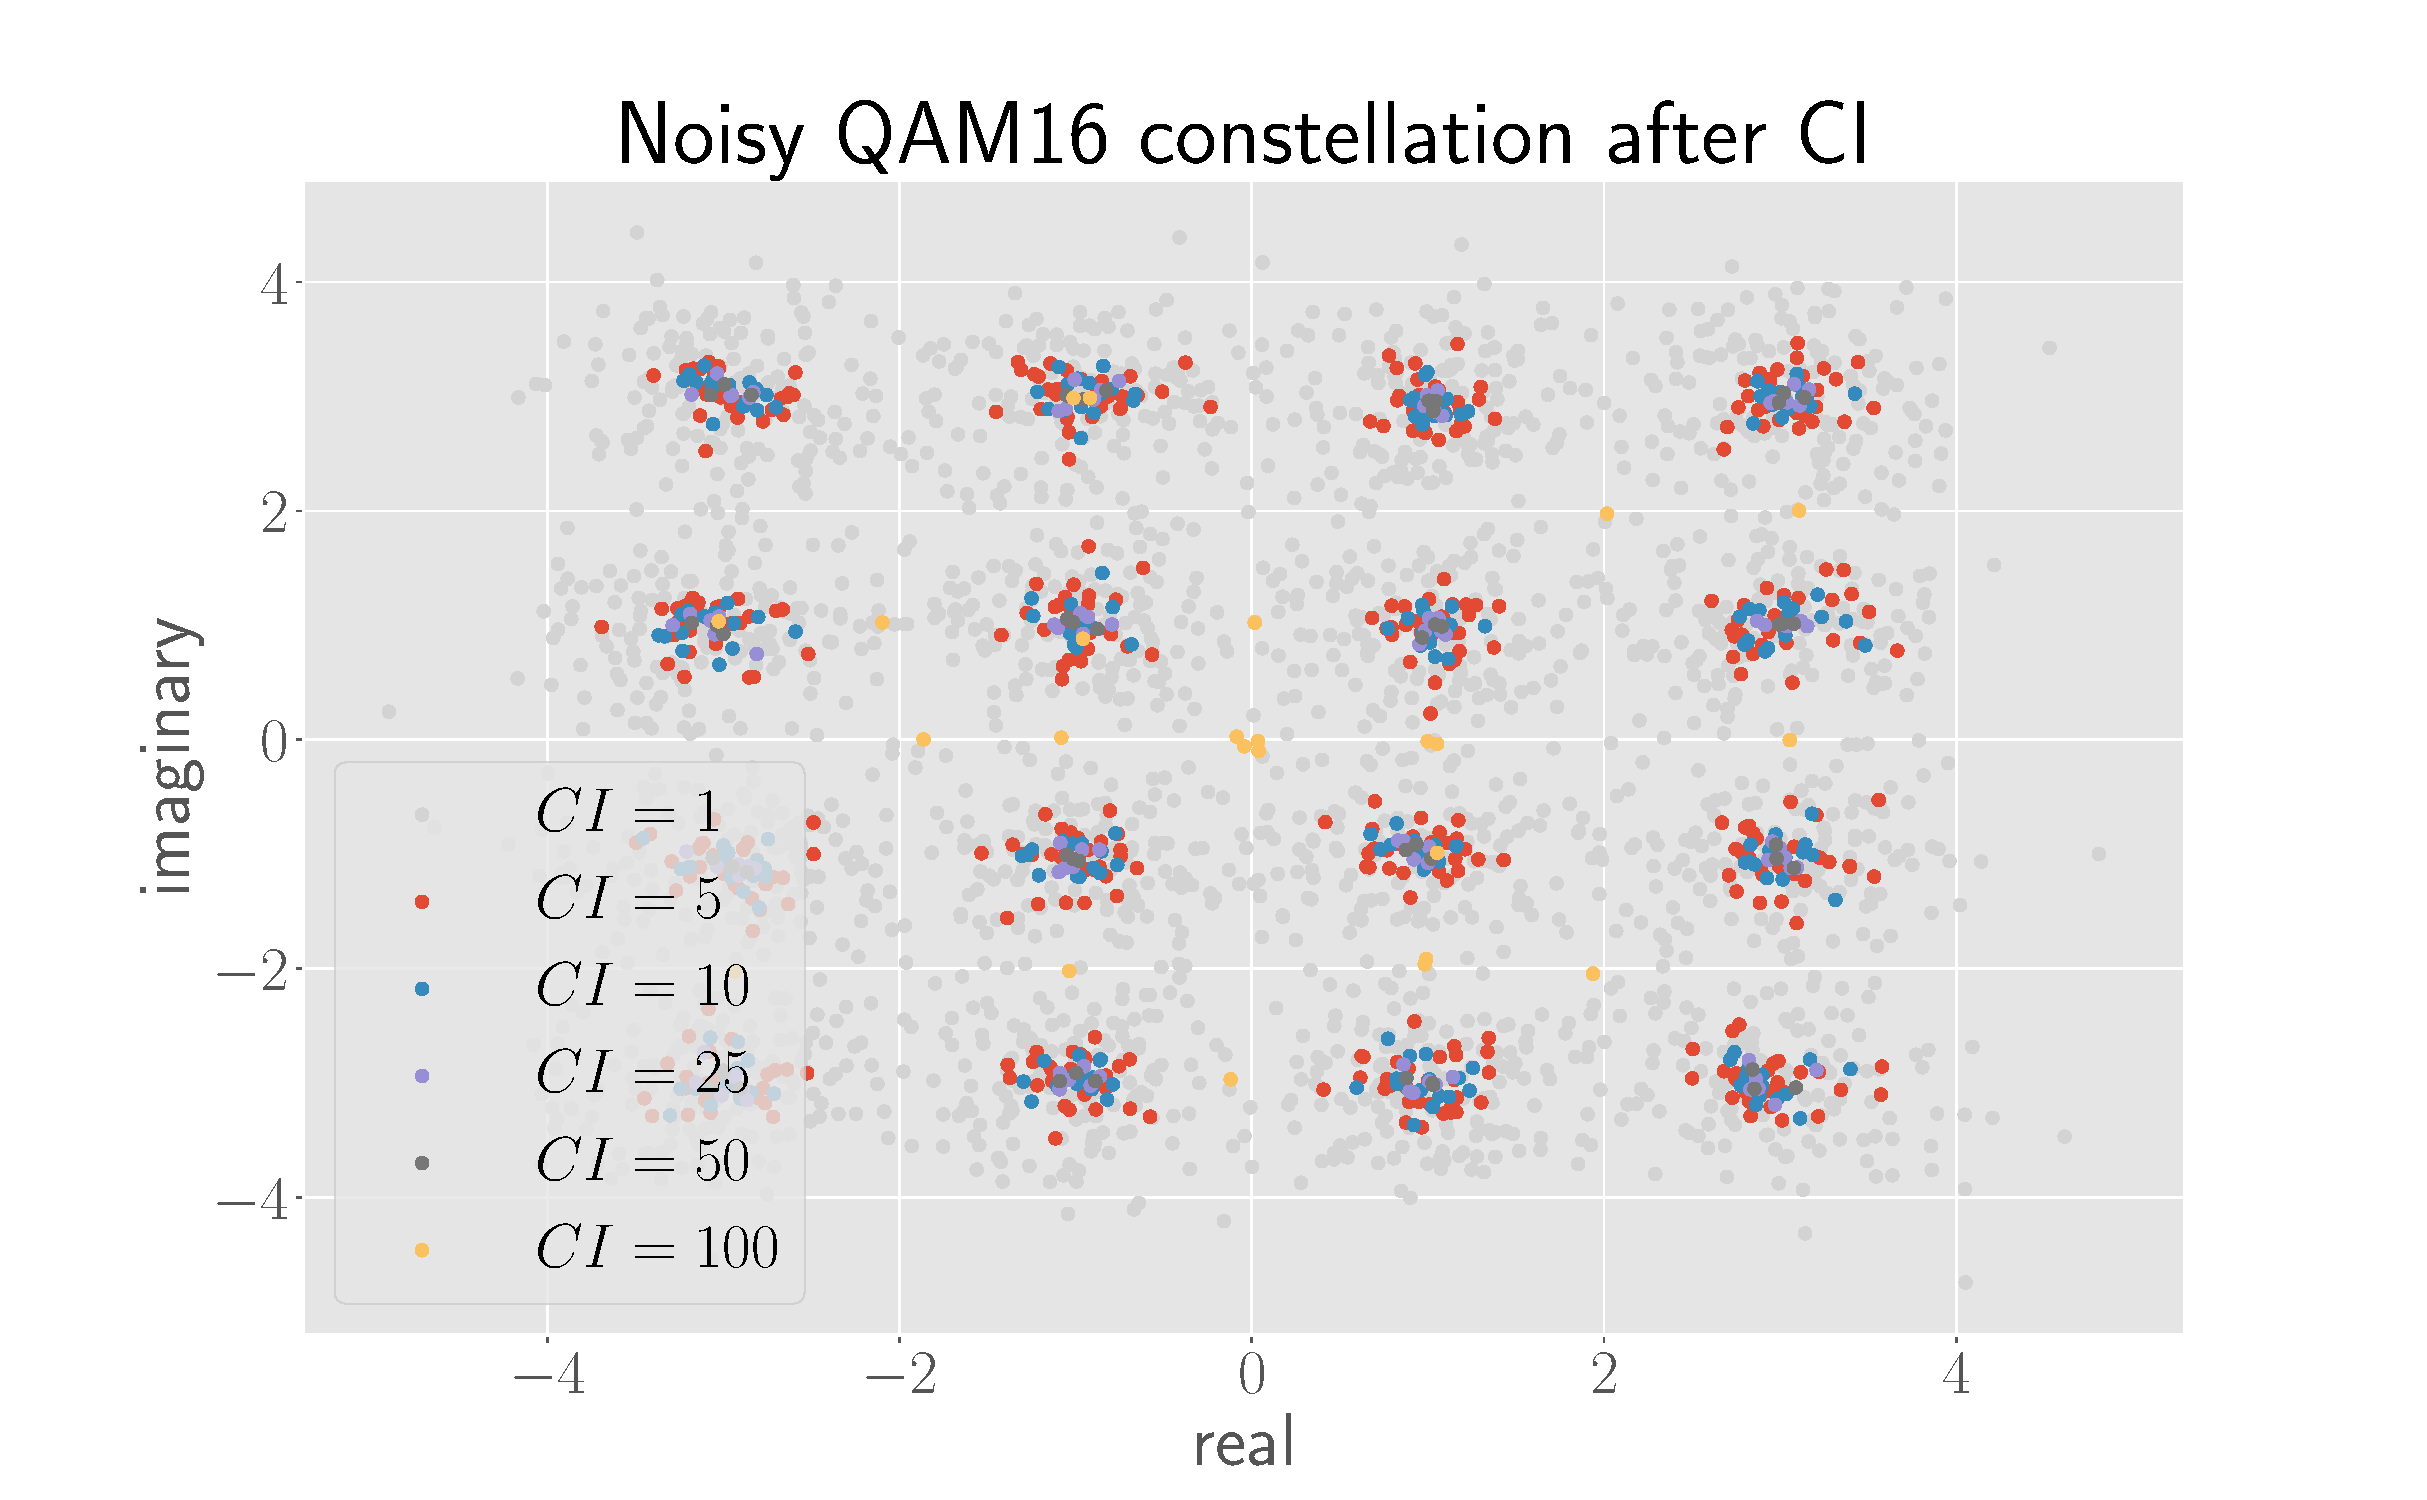
\includegraphics[width=1\textwidth]{graphics/ci_constellation.pdf} % first figure itself
        \caption{Constellation after coherent integration}\label{fig:ci_const}
    \end{minipage}\hfill
    \begin{minipage}{0.5\textwidth}
        \centering
        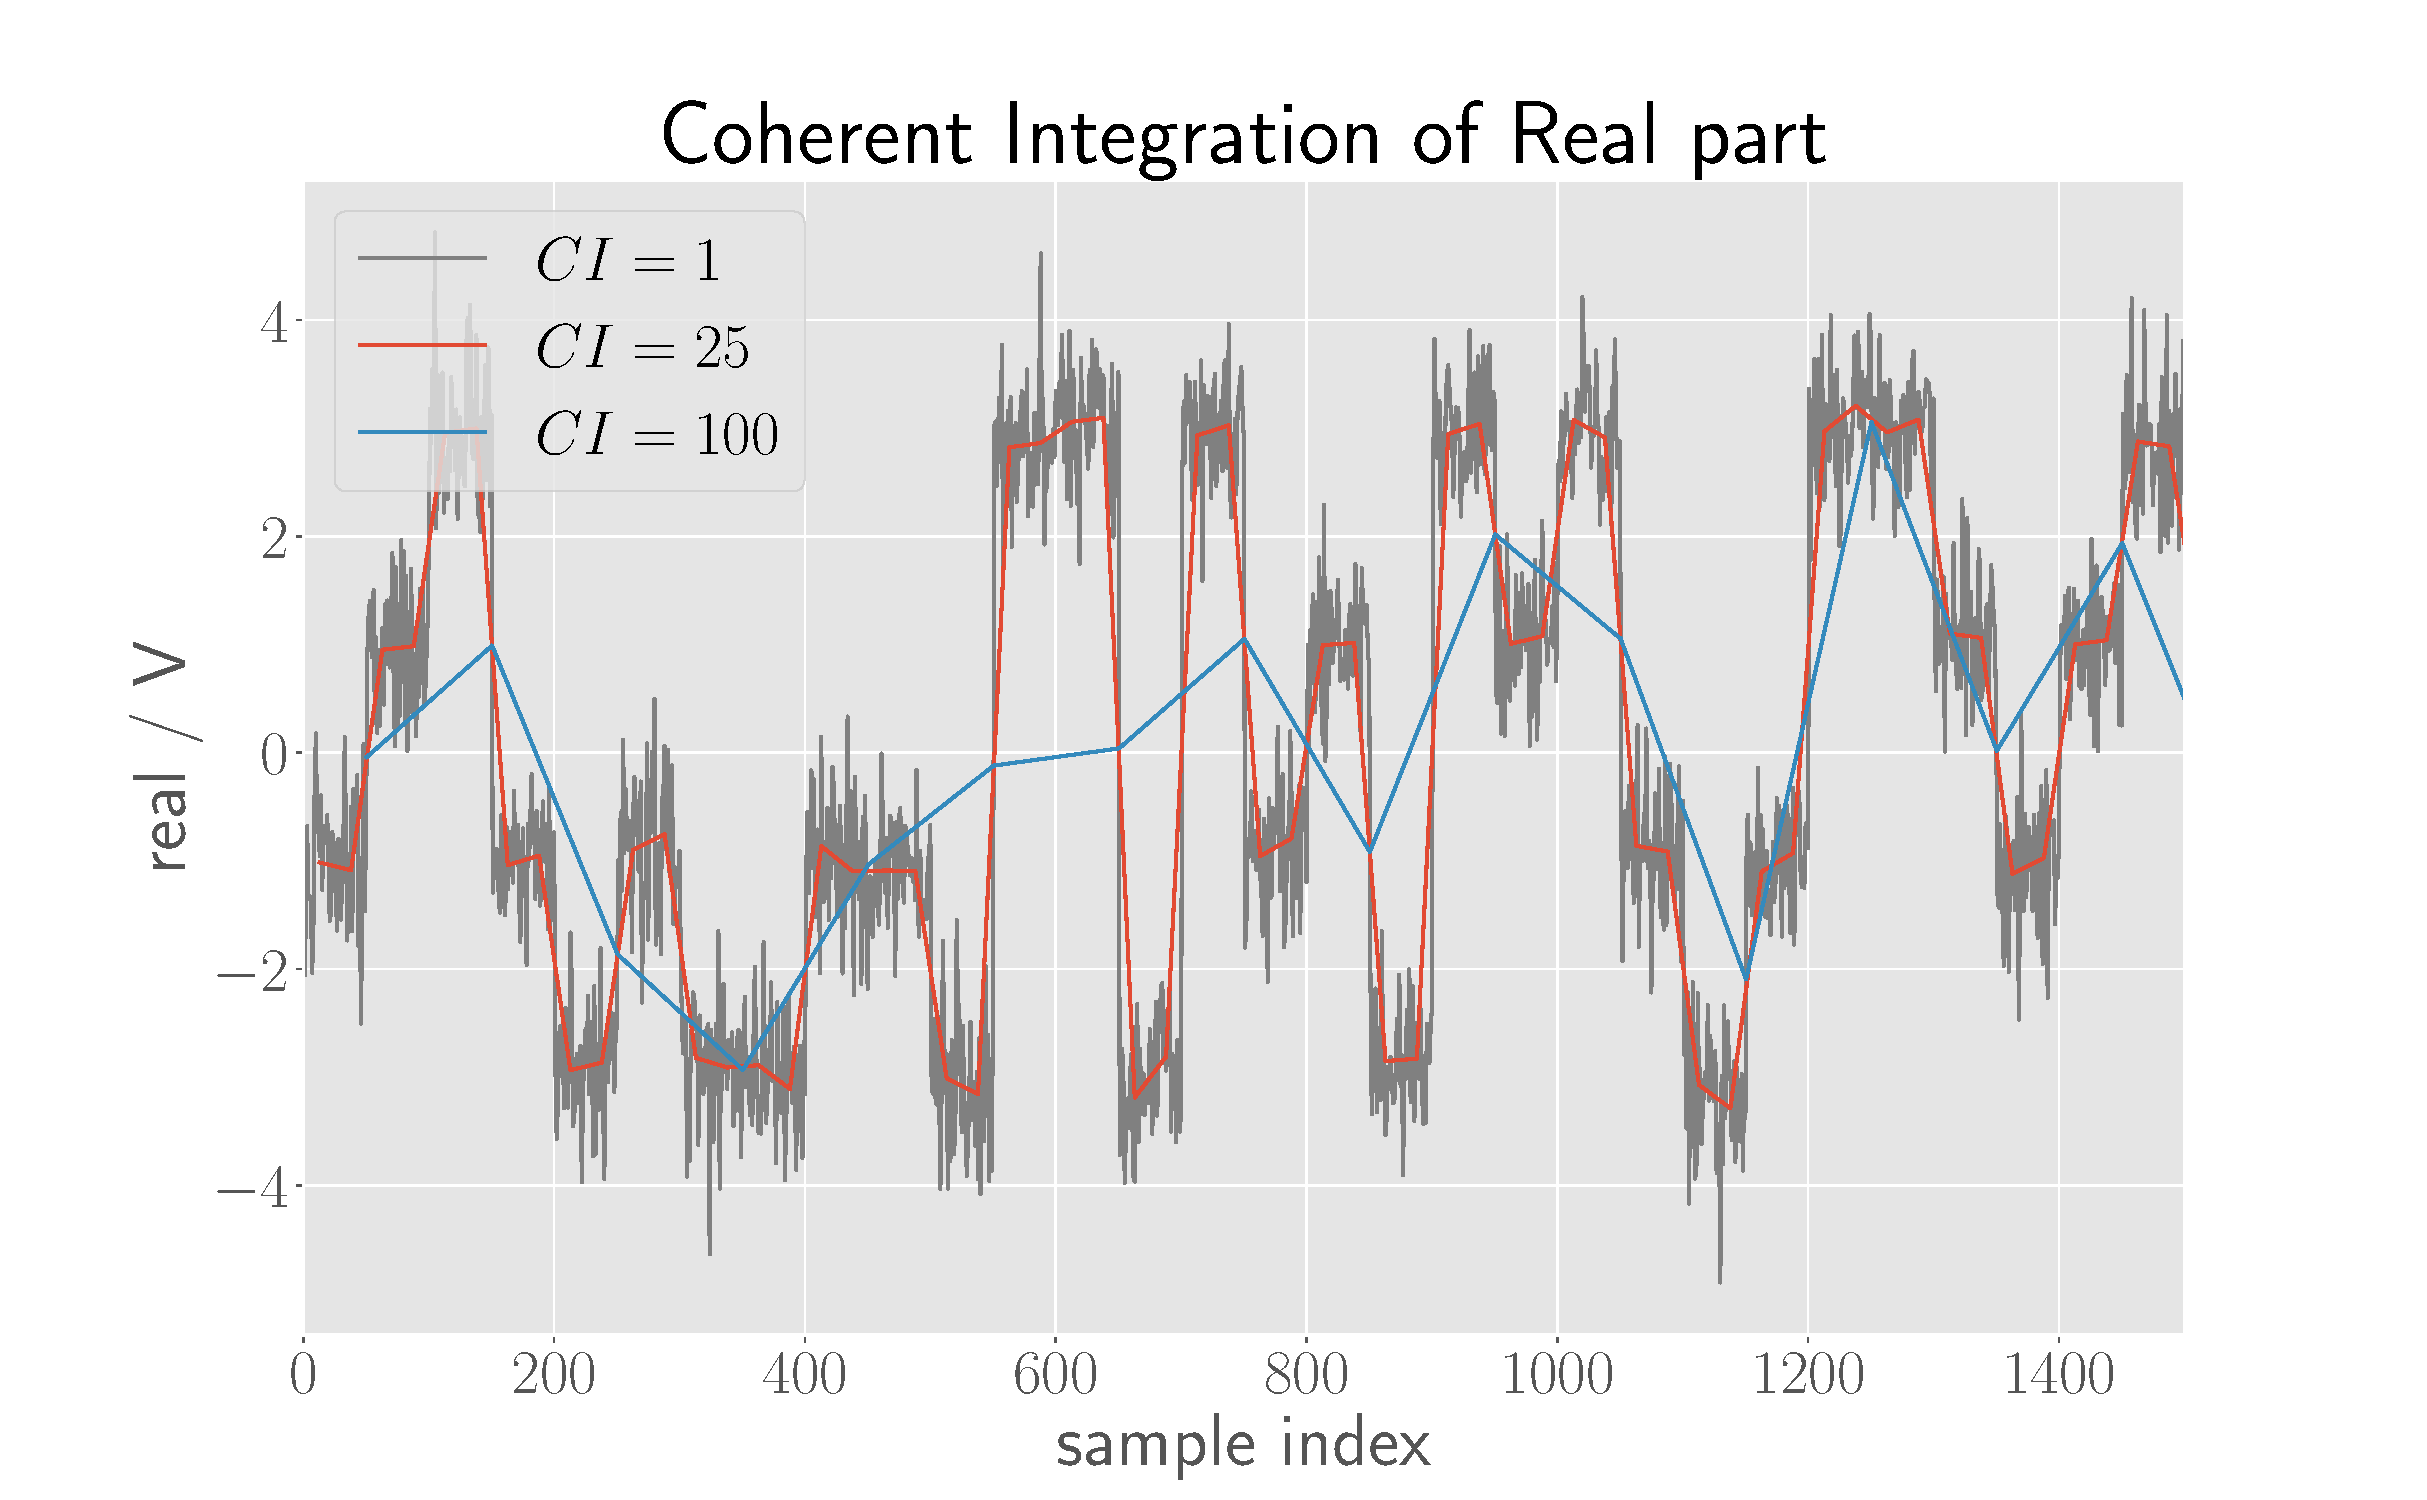
\includegraphics[width=1\textwidth]{graphics/ci_real.pdf} % second figure itself
        \caption{Real part after coherent integration.}\label{fig:ci_real}
    \end{minipage}
\end{figure}

As for the SNR, the noise power rises with $N$ but the signal power rises with $N^{2}$ resulting in an SNR increase which is proportional to the number of integrations. \cite{richards_pdf} Figure \ref{fig:snr_coh} confirms this linear relationship. In figure \ref{fig:snr_coh}, the value at $CI = 100$ is misleading, though. The difference used for the SNR calculation might be high but the actual samples are erroneous which further confirms the fact about the length of the integration period.

